\documentclass[11pt,fullpage]{article}
%\usepackage{multicol,wrapfig,amsmath,subfigure}
\usepackage{amsmath}
\usepackage{amsfonts,amssymb}
\usepackage{amsthm}
\usepackage{graphics,graphicx}
\usepackage{hyperref}
\usepackage[right = 2.5cm, left=2.5cm, top = 2.5cm, bottom =2.5cm]{geometry}
\pagestyle{plain}
\def\urlfont{\DeclareFontFamily{OT1}{cmtt}{\hyphenchar\font='057}
	\normalfont\ttfamily \hyphenpenalty=10000}

\newcommand*{\plogo}{\fbox{$\mathcal{PL}$}}
\newcommand{\norm}[1]{\|#1\|}
\newcommand{\innprod}[1]{\langle #1 \rangle}
\newcommand{\Tau}{\mathcal{T}}
\newcommand{\lap}{\Delta}
\newcommand{\problem}[1]{\paragraph{Problem #1}}
%\input macros
\newcommand{\deriv}{\mbox{d}}
\newcommand{\Real}{\mathbb R}
\newcommand{\eps}{\epsilon}
\newcommand{\Complex}{\mathbb C}
\newcommand{\abs}[1]{\left\vert#1\right\vert}
\newcommand{\set}[1]{\left\{#1\right\}}
\newcommand{\subheading}[1]{\noindent \textbf{#1}}
\newcommand{\grad}{\nabla}
\newcommand{\diver}{\textup{div} }
\newcommand{\jump}[1]{[#1]}
\newcommand{\limit}[2]{\lim_{#1 \rightarrow #2}}
\newcommand{\mollify}[1]{ \mathcal{J}_\epsilon #1 }
\newcommand{\conv}[2]{#1 \ast #2}
\newcommand{\D}{D}
\newcommand{\K}{\mathcal{K}}
\newcommand{\C}{\mathcal{C}}
\newcommand{\Torus}{\mathbb{T}}
\newcommand{\Integer}{\mathbb{Z}}
\newcommand{\Naturals}{\mathbb{N}}
\newcommand{\ineqtext}[1]{ ^{\text{\tiny #1}}}
\newcommand{\F}{\mathcal{F}}
\newcommand{\bx}{\mathbf{x}}
\newcommand{\by}{\mathbf{y}}
\newcommand{\intab}{\int_{a}^{b}}
\newcommand{\intom}{\int_{\Omega}}
\newcommand{\Ltwo}{{L^2}}
\newcommand{\Ltwoom}{{L^2(\Omega)}}
\newcommand{\Linf}{{L^\infty}}
\newcommand{\Linfom}{{L^\infty(\Omega)}}
\renewcommand{\i}{{i}}
\newcommand{\ip}{{i+1}}
\newcommand{\ipp}{{i+2}}
\newcommand{\im}{{i-1}}
\newcommand{\imm}{{i-2}}
\renewcommand{\j}{{j}}
\newcommand{\jp}{{j+1}}
\newcommand{\jpp}{{j+2}}
\newcommand{\jm}{{j-1}}
\newcommand{\jmm}{{j-2}}
\newcommand{\n}{{n}}
\newcommand{\np}{{n+1}}
\newcommand{\npp}{{n+2}}
\newcommand{\nm}{{n-1}}
\newcommand{\nmm}{{n-2}}

%Nancy's macros
\newcommand{\reg}[1]{#1^\epsilon}
\newcommand{\Lpr}[1]{L^{#1}(\mathbb{R}^n)}
\newcommand{\Lp}[1]{L^{#1}(\Omega)}
\newcommand{\intreal}[1]{\int_{\mathbb{R}^{#1}}\hspace{-8pt}}
\newcommand{\modenergy}{\mathcal{E}_H}
\newcommand{\ball}{B_n}
\newcommand{\balltime}{B_n\times [0,T]}

\newtheorem{theorem}{Theorem}
\theoremstyle{lemma}
\newtheorem{prop}{Proposition}
\newtheorem{proposition}{Proposition}
\newtheorem{corollary}{Corollary}
\theoremstyle{definition}
\newtheorem{definition}{Definition}
\newtheorem{exercise}{Exercise}
\newtheorem{algorithm}{Algorithm}
\newtheorem{question}{Question}
%\theoremstyle{remark}
\newtheorem{remark}{Remark}
\newtheorem{rmk}{Remark}
\newtheorem{example}{Example}
\theoremstyle{lemma}
\newtheorem{lemma}{Lemma}

\begin{document}
	
	\begin{center}
		\textbf{\Large{deal.II Example Code Documentation}}
		\\
		\textbf{\Large{AMSC663}} \\ 
		\textbf{\large{Gareth Johnson}}
		\\
		\today
	\end{center}

In order to learn the functionality of deal.II, I followed various example programs found in deal.II's tutorial \cite{DealIITut}. Each tutorial focused on introducing various functionality in the library. For each tutorial that I completed, I will document the PDE that it solved as well as discuss some of the particular functionality that was learned and how it can be used in my own code.

\section*{Step-1}
In this tutorial we learned how to generate both a rectangular and circular mesh. It also demonstrated how to globally refine the mesh and how to export a plot of the mesh to a file. Below are plots of each mesh after 5 levels of global refinement.

\begin{figure}[!ht]
	\begin{minipage}{.4\paperwidth}
		\centering
		
\includegraphics[scale=.45]{Step1-1.png}
	\end{minipage}%
	\begin{minipage}{.4\paperwidth}
		\centering
		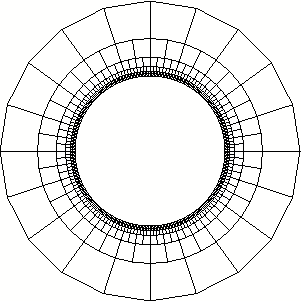
\includegraphics[scale=.45]{Step1-2.png}
	\end{minipage}
\end{figure}

\section*{Step-2}
In this tutorial we learned how to distribute degree of freedoms (DoFs) for a given finite element type and a given triangulation. In addition, we learned how to renumber the DoF using the Cuthill Mckee front marching algorithm in order for the DoFs to lie closer to the diagonal of the matrix, which can benefit certain solvers. Below are visual representations of the sparsity pattern with and without renumbering the DoFs.

\begin{figure}[!ht]
	\begin{minipage}{.4\paperwidth}
		\centering
		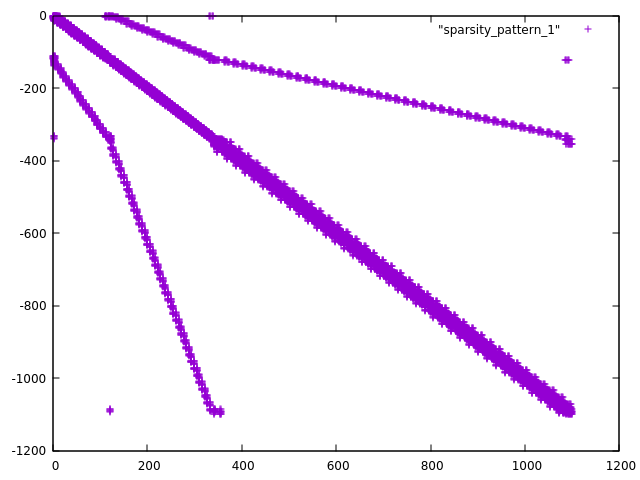
\includegraphics[scale=.45]{Step2-1.png}
	\end{minipage}%
	\begin{minipage}{.4\paperwidth}
		\centering
		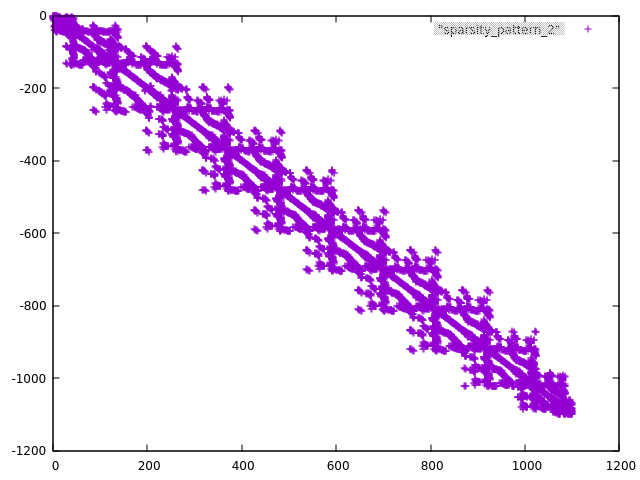
\includegraphics[scale=.45]{Step2-2.png}
	\end{minipage}
\end{figure}

\section*{Step-3}
In this tutorial we solved Poisson's equation:
$$
\begin{cases}
-\lap u = f(x) &\text{in }\Omega,\\
u = 0 & \text{on }\partial\Omega,
\end{cases}
$$
where $f(x) = 1$ and $\Omega = [0,1]^2$. This was the first program where we actually solved a PDE. We learned how to take the triangulation and DoFs that were computed in Step--2 and actually apply them to compute the bilinear and right hand side of the equation using $Q_1$ elements and how to incorporate dirichlet boundary conditions. We also learned how to interface with linear algebra routines, such as CG, in order to actually solve the system. Finally, it demonstrated how to export the solution into various graphical formats to view. Below are two such visual representations of the solution.

\begin{figure}[!ht]
	\begin{minipage}{.4\paperwidth}
		\centering
		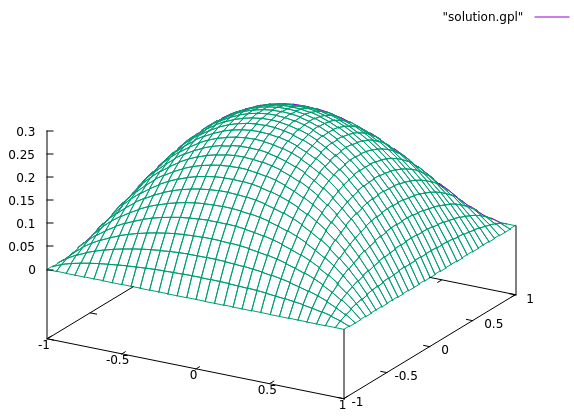
\includegraphics[scale=.45]{Step3-gnuplot.png}
	\end{minipage}%
	\begin{minipage}{.4\paperwidth}
		\centering
		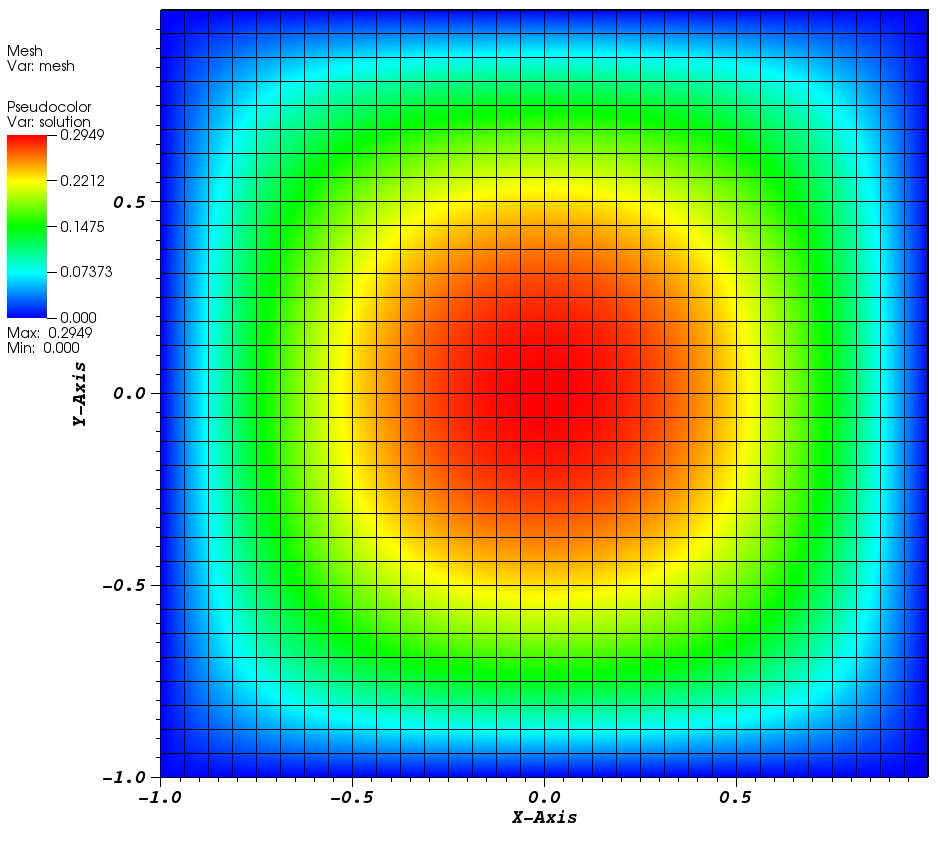
\includegraphics[scale=.7]{Step3-visit.png}
	\end{minipage}
\end{figure}
\clearpage
\section*{Step-4}
In this tutorial we solved Poisson's equation:
$$
\begin{cases}
-\lap u = f(x) &\text{in }\Omega,\\
u = g(x) & \text{on }\partial\Omega,
\end{cases}
$$
where 
$$
f(x) = \begin{cases}
4(x^4 + y^4) & \text{if } \Omega \subset \Real^2\\
4(x^4 + y^4 + z^4) & \text{if } \Omega \subset \Real^3\\
\end{cases}, \quad 
g(x) = \begin{cases}
x^2 + y^2 & \text{if } \Omega \subset \Real^2\\
x^2 + y^2 + z^2 & \text{if } \Omega \subset \Real^3\\
\end{cases},
$$ and $\Omega$ is the unit square or cube. The new features of this example were how to take advantage of deal.II's dimensionless programming technique. By using C++'s template feature, it allows us to write the code where the dimension is a compile time parameter. This feature allows us to change the dimension of the PDE with almost no modifications to the actual code. In addition, it showed how to implement non-constant forcing functions and dirichlet boundary conditions. Below are plots of the solution in both 2D and 3D.

\begin{figure}[!ht]
	\centering
	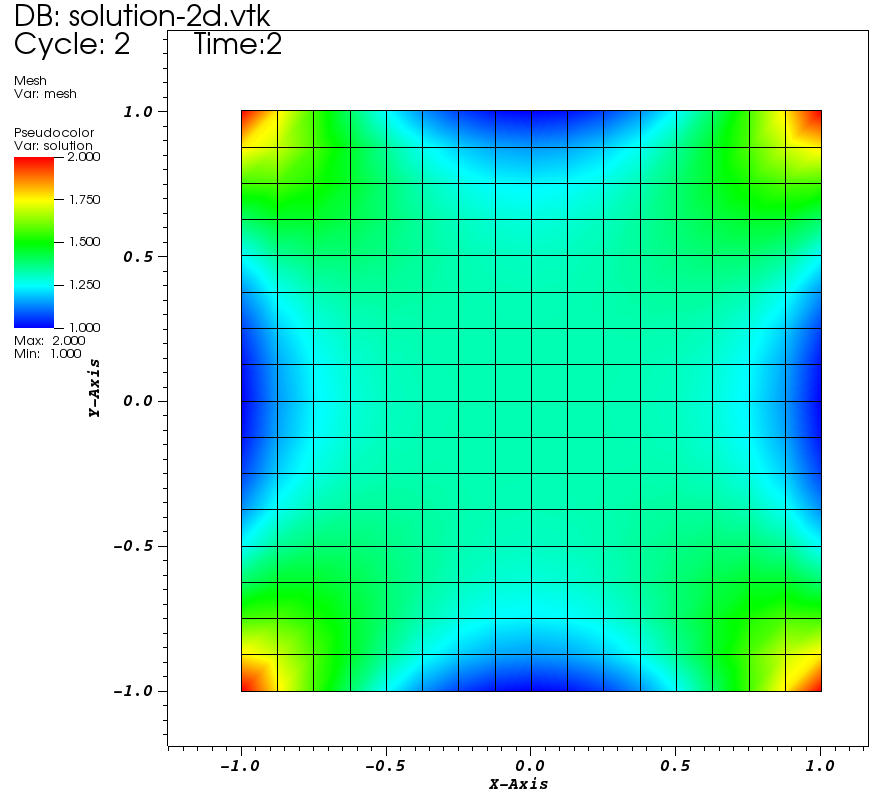
\includegraphics[scale=.7]{Step4-2d.png}
\end{figure}

\begin{figure}[!ht]
	\begin{minipage}{.4\paperwidth}
		\centering
		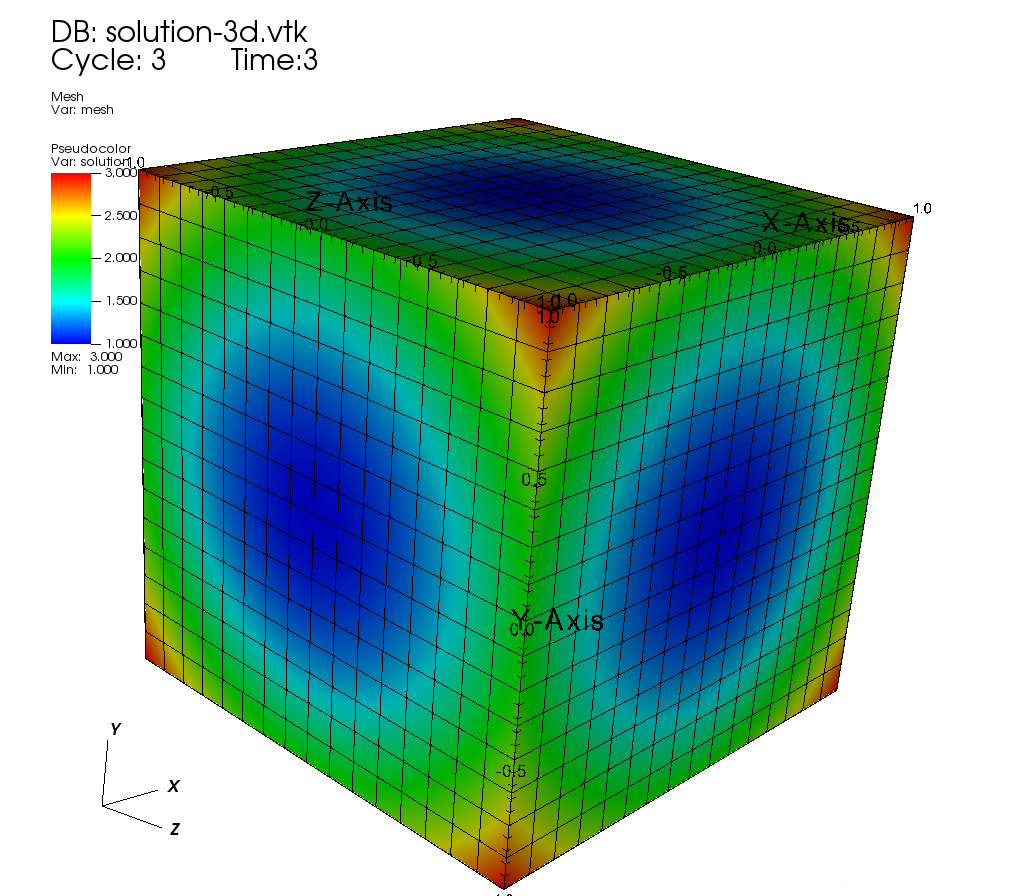
\includegraphics[scale=.7]{Step4-3d.png}
	\end{minipage}%
	\begin{minipage}{.4\paperwidth}
		\centering
		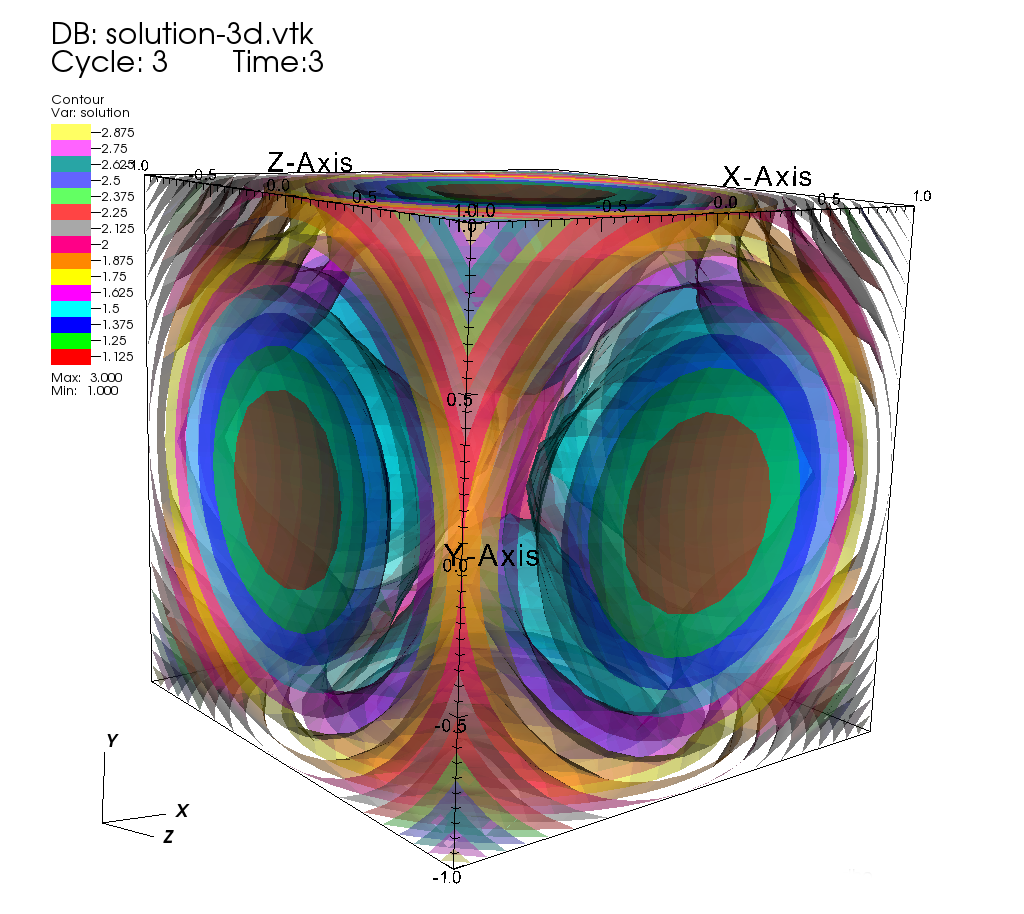
\includegraphics[scale=.7]{Step4-3dcon.png}
	\end{minipage}
\end{figure}
\clearpage

\section*{Step-5}
In this tutorial we solved an elliptic equation of the form:
$$
\begin{cases}
-\grad \cdot(a(x)\grad u(x)) = 1 &\text{in }\Omega,\\
u = 0 & \text{on }\partial\Omega,
\end{cases}
$$
where $\Omega = B(0,1)$ and 
$$
a(x) = \begin{cases}
20 & \text{if }\abs{x} < 0.5\\
1 & \text{otherwise}
\end{cases}.
$$ 
The new functionality introduced was how to incorporate non-constant coefficients into the bilinear form, how to use preconditioning (specifically SSOR) when using an iterative solver such as CG, and how to solve the problem on a sequence of globally refined meshes. Below are plots of the solution on increasingly refined meshes.

\begin{figure}[!ht]
	\begin{minipage}{.45\paperwidth}
		\centering
		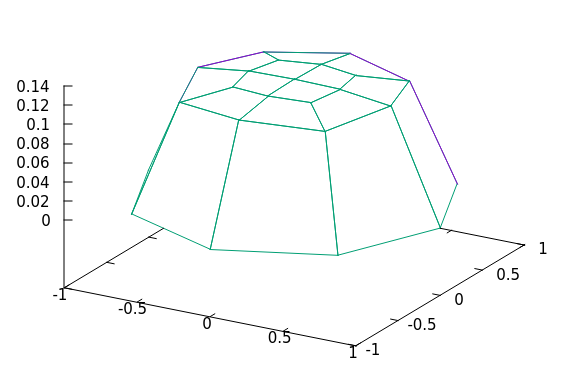
\includegraphics[scale=.5]{Step5-1.png}
	\end{minipage}%
	\begin{minipage}{.4\paperwidth}
		\centering
		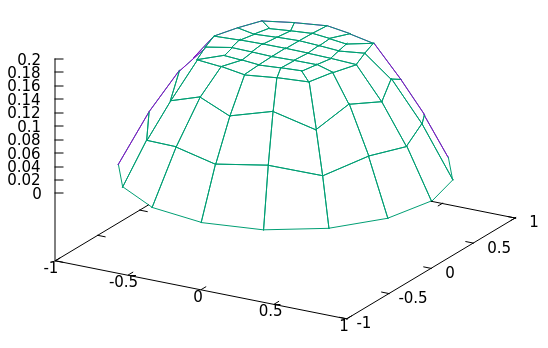
\includegraphics[scale=.5]{Step5-2.png}
	\end{minipage}
	\begin{minipage}{.45\paperwidth}
		\centering
		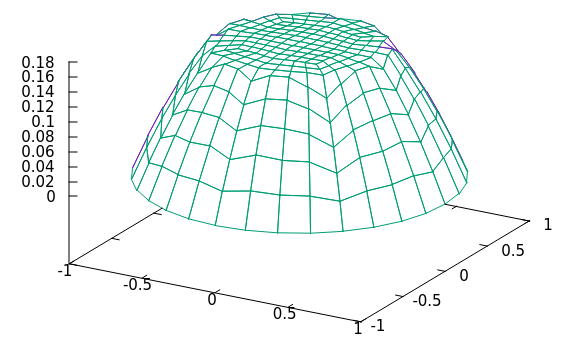
\includegraphics[scale=.5]{Step5-3.png}
	\end{minipage}%
	\begin{minipage}{.4\paperwidth}
		\centering
		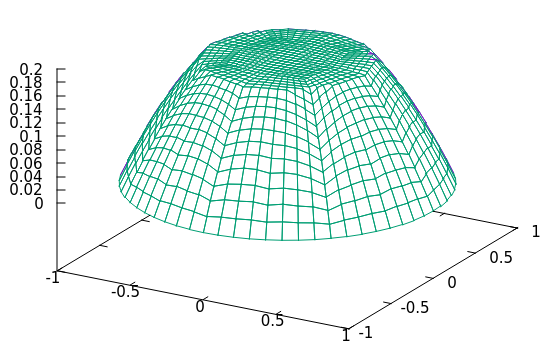
\includegraphics[scale=.5]{Step5-4.png}
	\end{minipage}
\end{figure}

\section*{Step-6}
In this tutorial we solved the same PDE as in Step-5:
$$
\begin{cases}
-\grad \cdot(a(x)\grad u(x)) = 1 &\text{in }\Omega,\\
u = 0 & \text{on }\partial\Omega,
\end{cases}
$$
where $\Omega = B(0,1)$ and 
$$
a(x) = \begin{cases}
20 & \text{if }\abs{x} < 0.5\\
1 & \text{otherwise}
\end{cases}.
$$
The main difference is that in this program we added the ability to adaptively refine/coarsen the mesh. This process works by first computing the Kelly error estimator on each element, then marking 30\% of the elements with the highest error to be refined and 3\% of the elements with the lowest error to be coarsened. There are some key things to point out about the refinement/coarsening procedure. First, the percentages chosen were arbitrary and can be easily tuned for specific problems. Second, the percentage of marked elements is not equivalent to the total percentage of elements that will be refined/coarsened. This is because elements are not allowed to be refined twice when neighbor elements are not refined. Lastly, since deal.II uses quadrilateral elements the process of refinement will cause there to be hanging nodes. The method of implementing these was also covered in the tutorial. Below are plots of the solution and mesh as we adaptively refined/coarsened the mesh.

\begin{figure}[!ht]
	\begin{minipage}{.45\paperwidth}
		\centering
		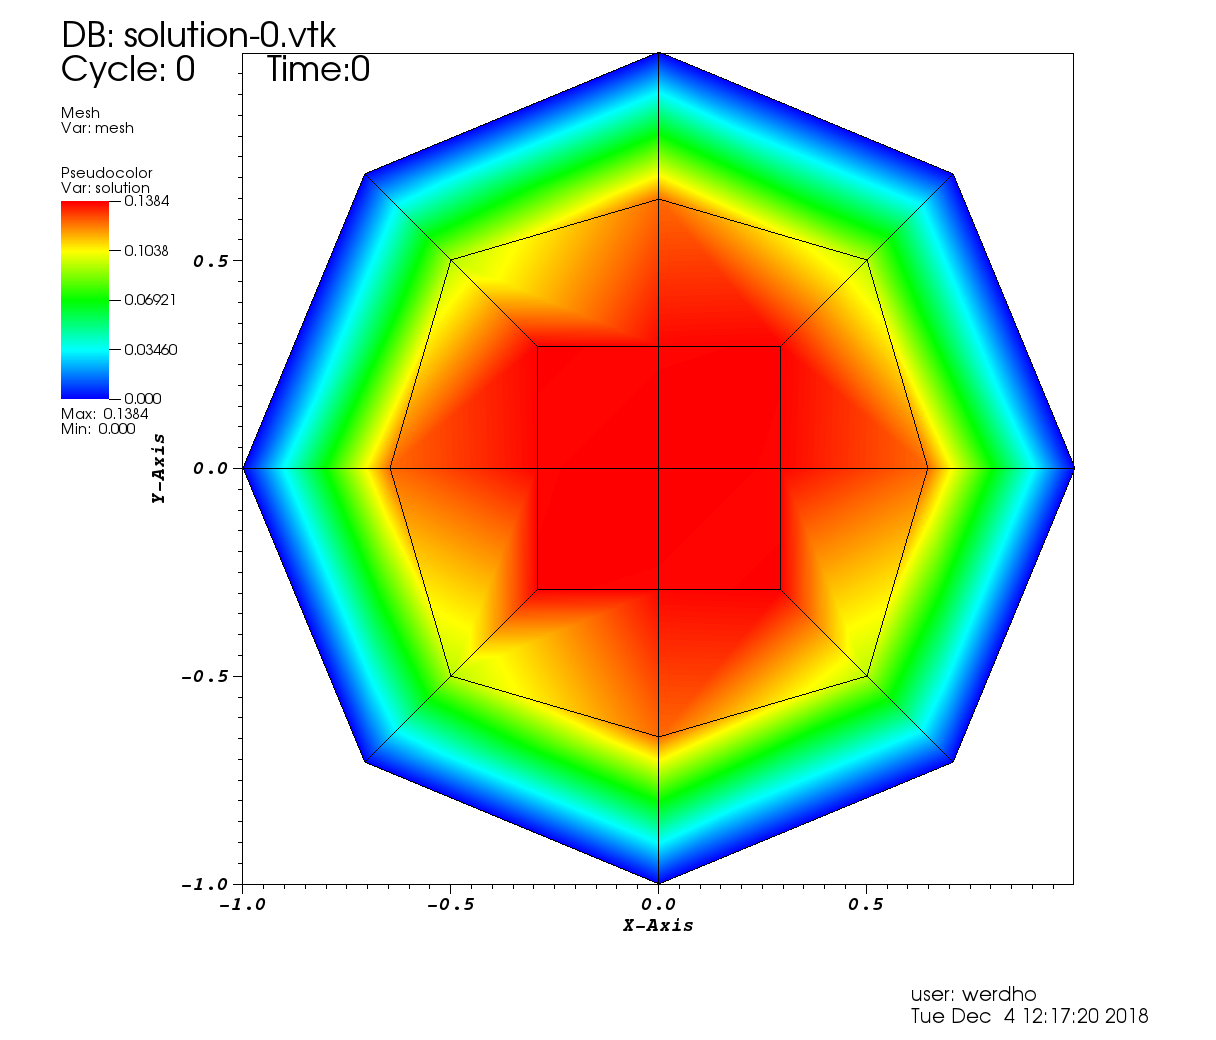
\includegraphics[scale=.12]{Step6-1.png}
	\end{minipage}%
	\begin{minipage}{.4\paperwidth}
		\centering
		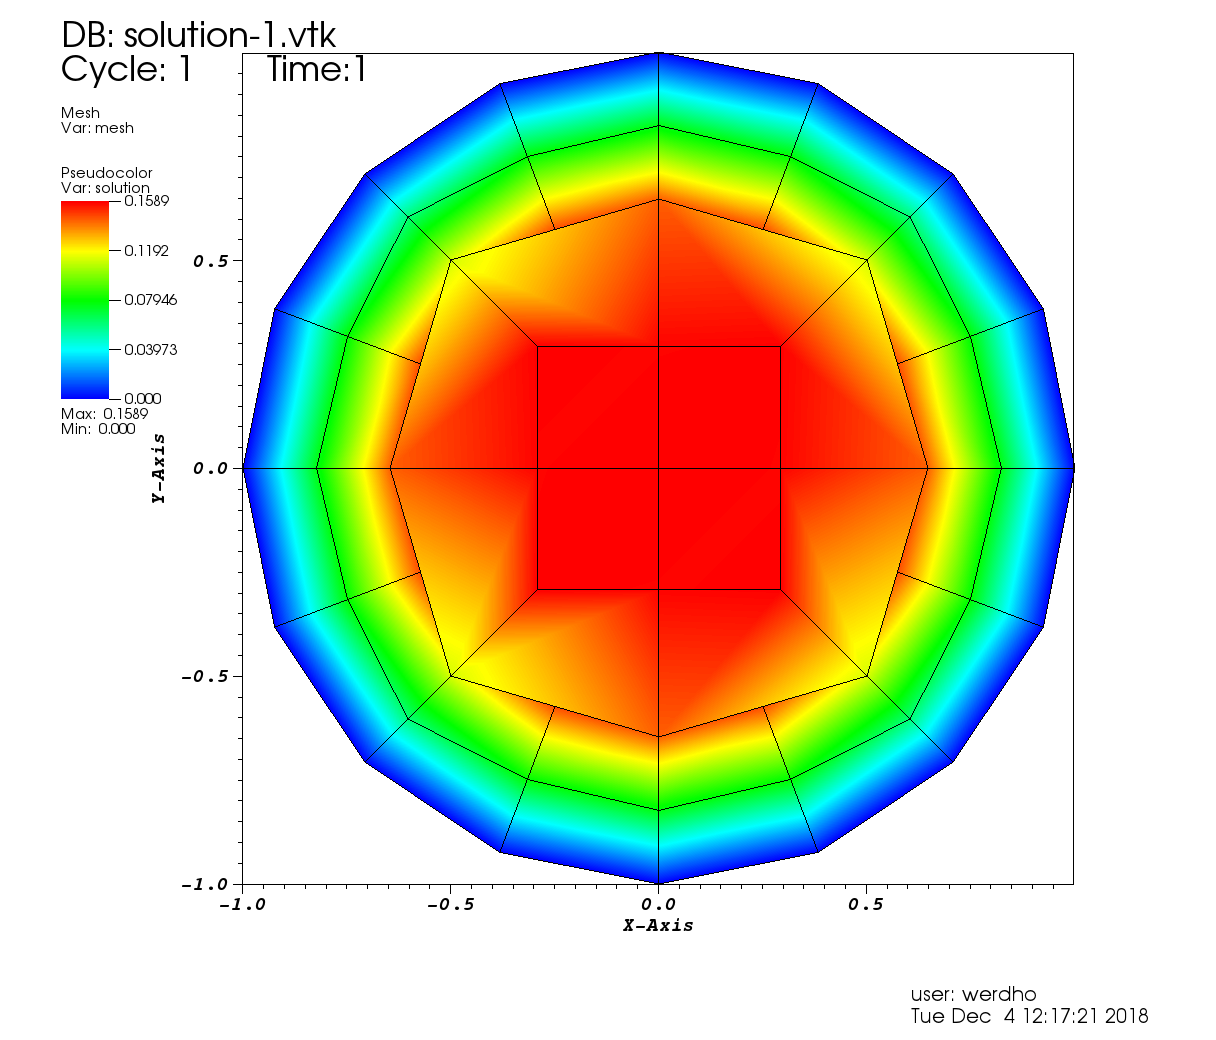
\includegraphics[scale=.12]{Step6-2.png}
	\end{minipage}
	\begin{minipage}{.45\paperwidth}
		\centering
		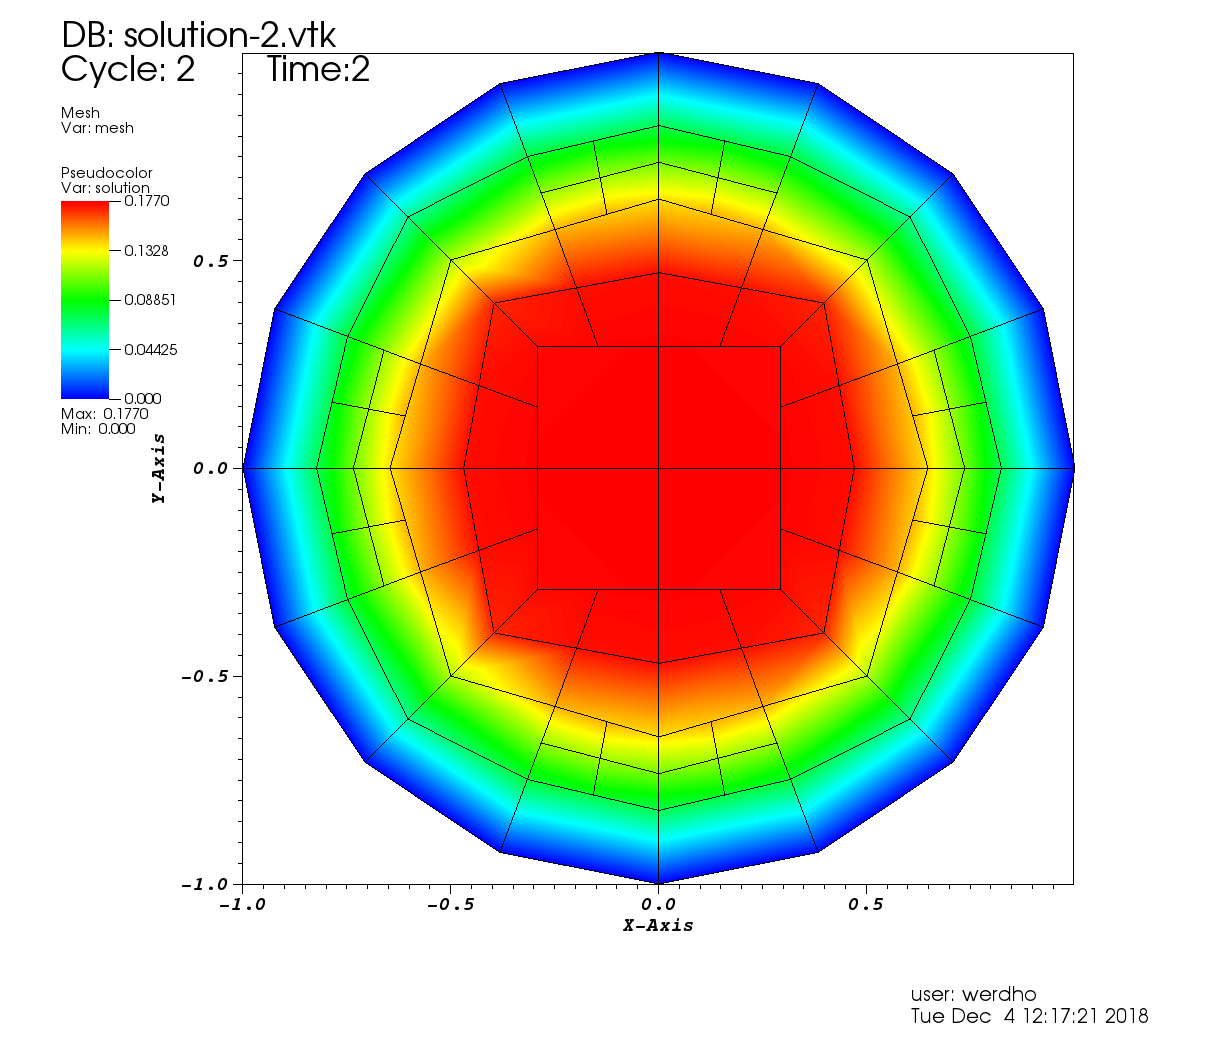
\includegraphics[scale=.12]{Step6-3.png}
	\end{minipage}%
	\begin{minipage}{.4\paperwidth}
		\centering
		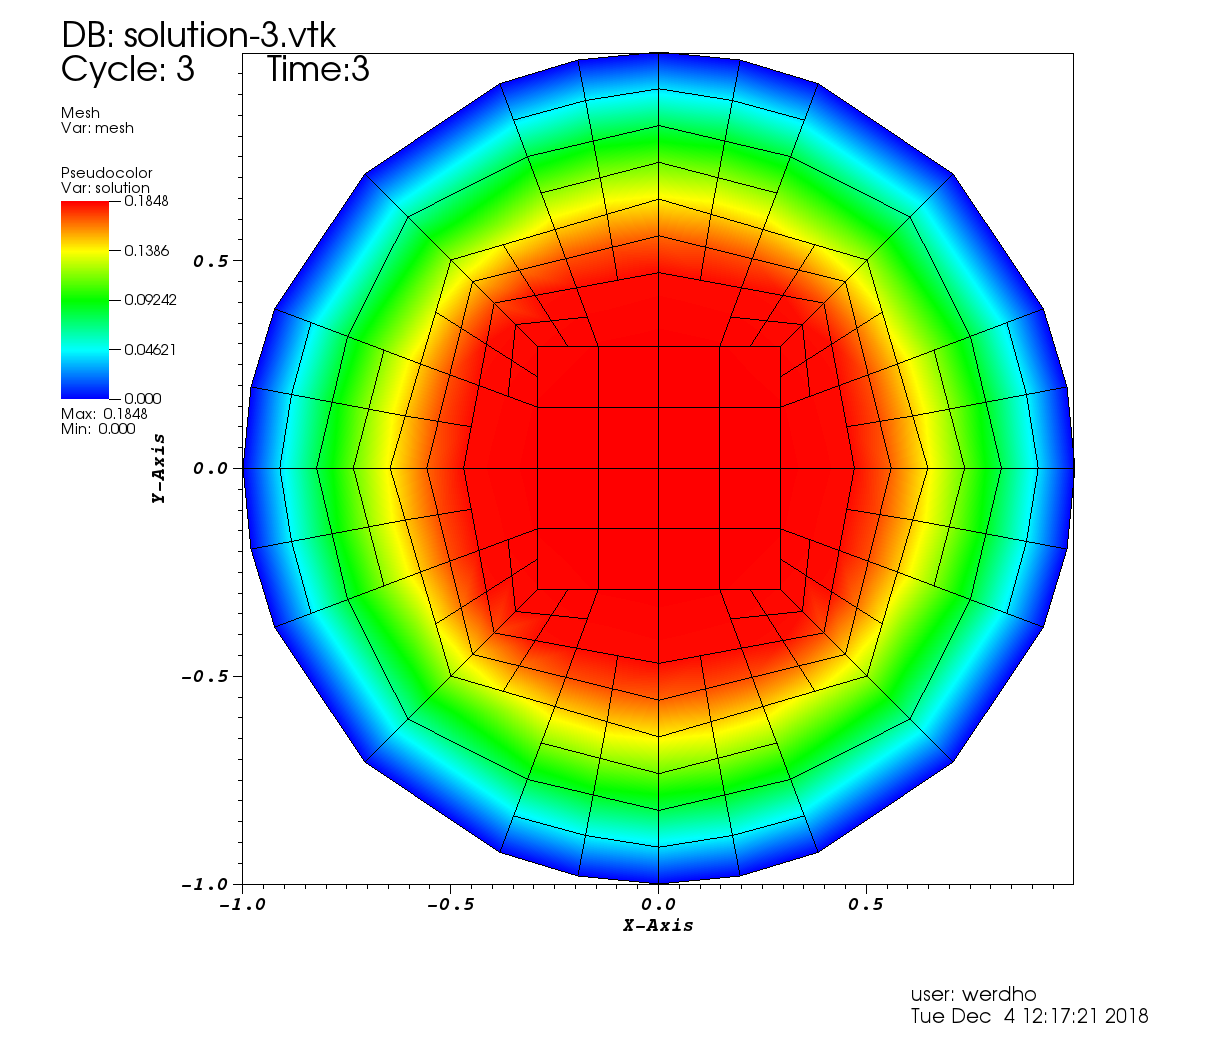
\includegraphics[scale=.12]{Step6-4.png}
	\end{minipage}
\end{figure}
\begin{figure}[!ht]
	\begin{minipage}{.45\paperwidth}
		\centering
		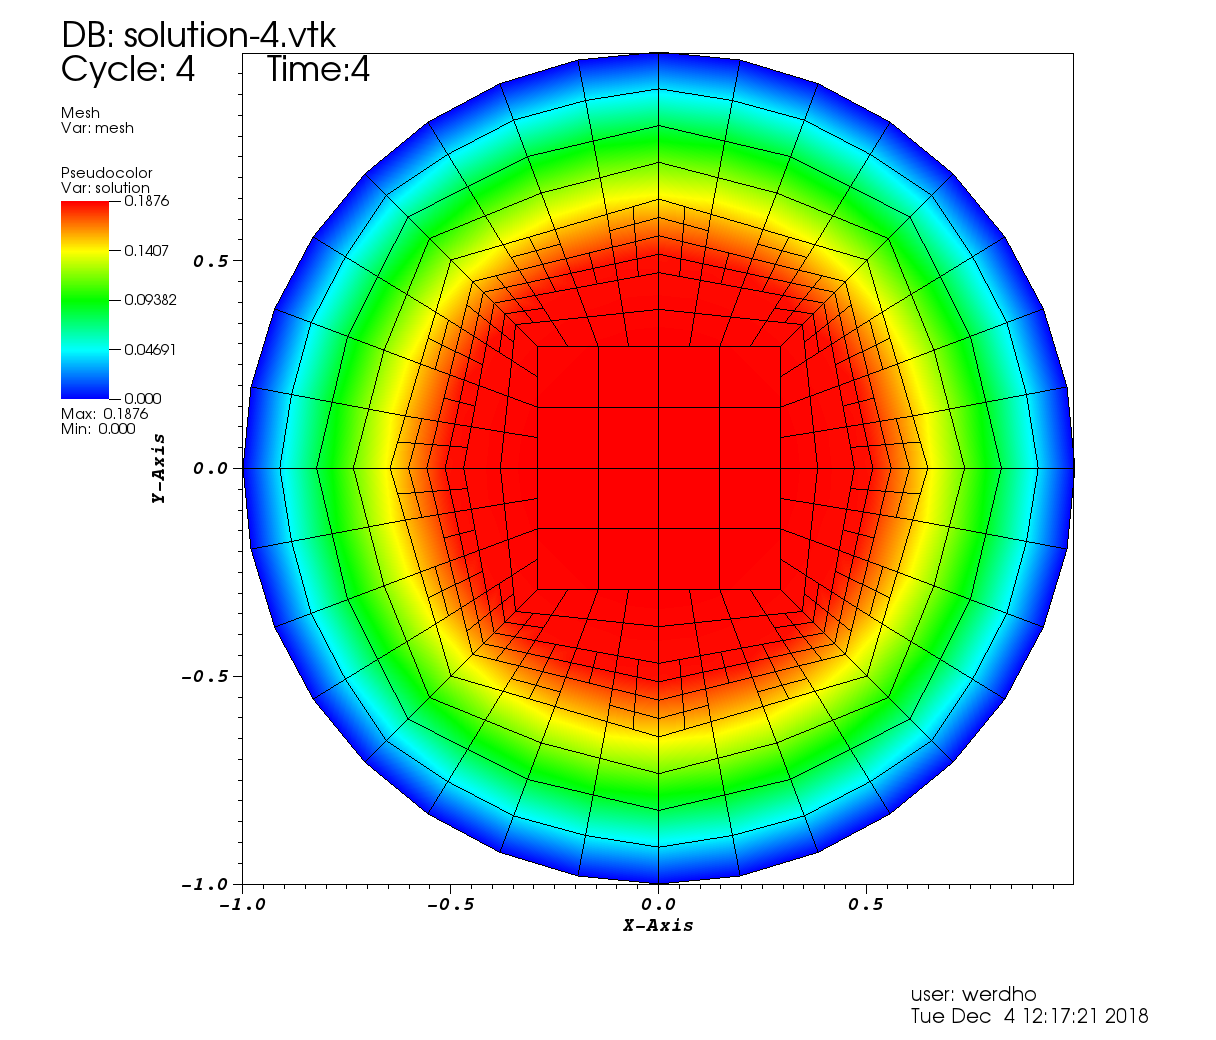
\includegraphics[scale=.12]{Step6-5.png}
	\end{minipage}%
	\begin{minipage}{.4\paperwidth}
		\centering
		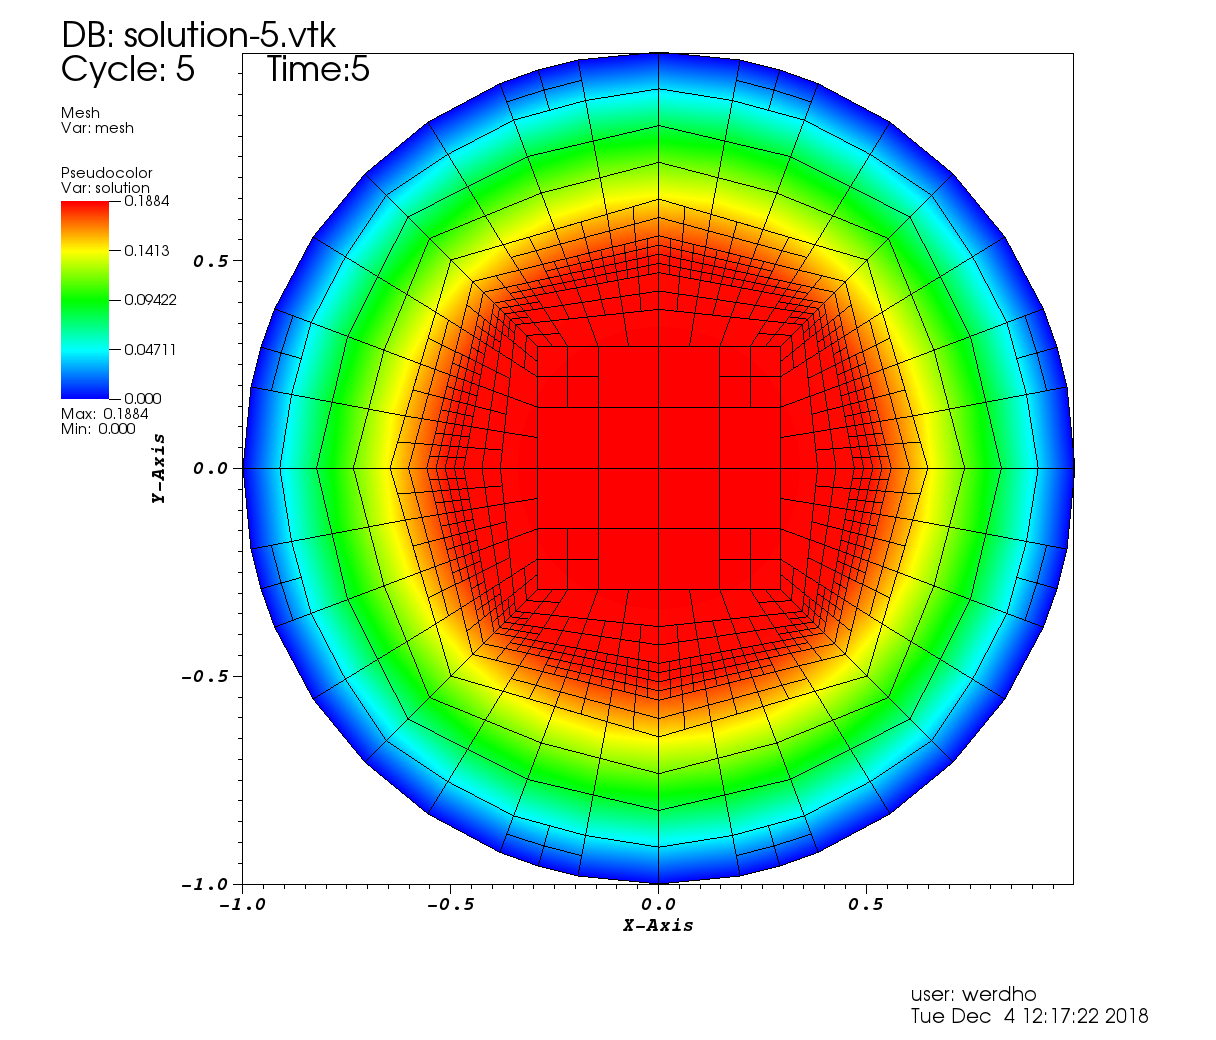
\includegraphics[scale=.12]{Step6-6.png}
	\end{minipage}
	\begin{minipage}{.45\paperwidth}
		\centering
		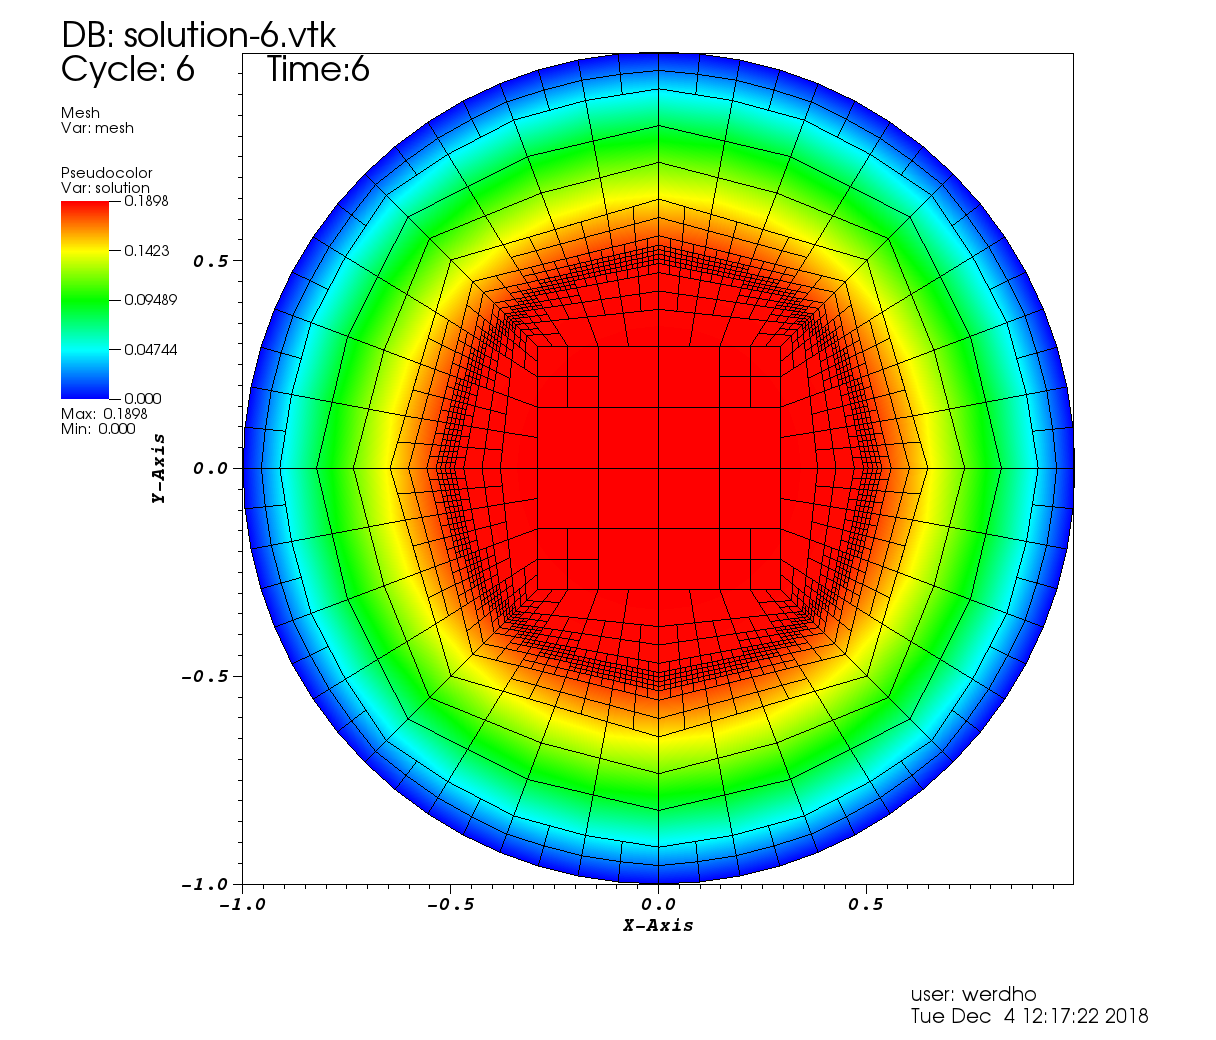
\includegraphics[scale=.12]{Step6-7.png}
	\end{minipage}%
	\begin{minipage}{.4\paperwidth}
		\centering
		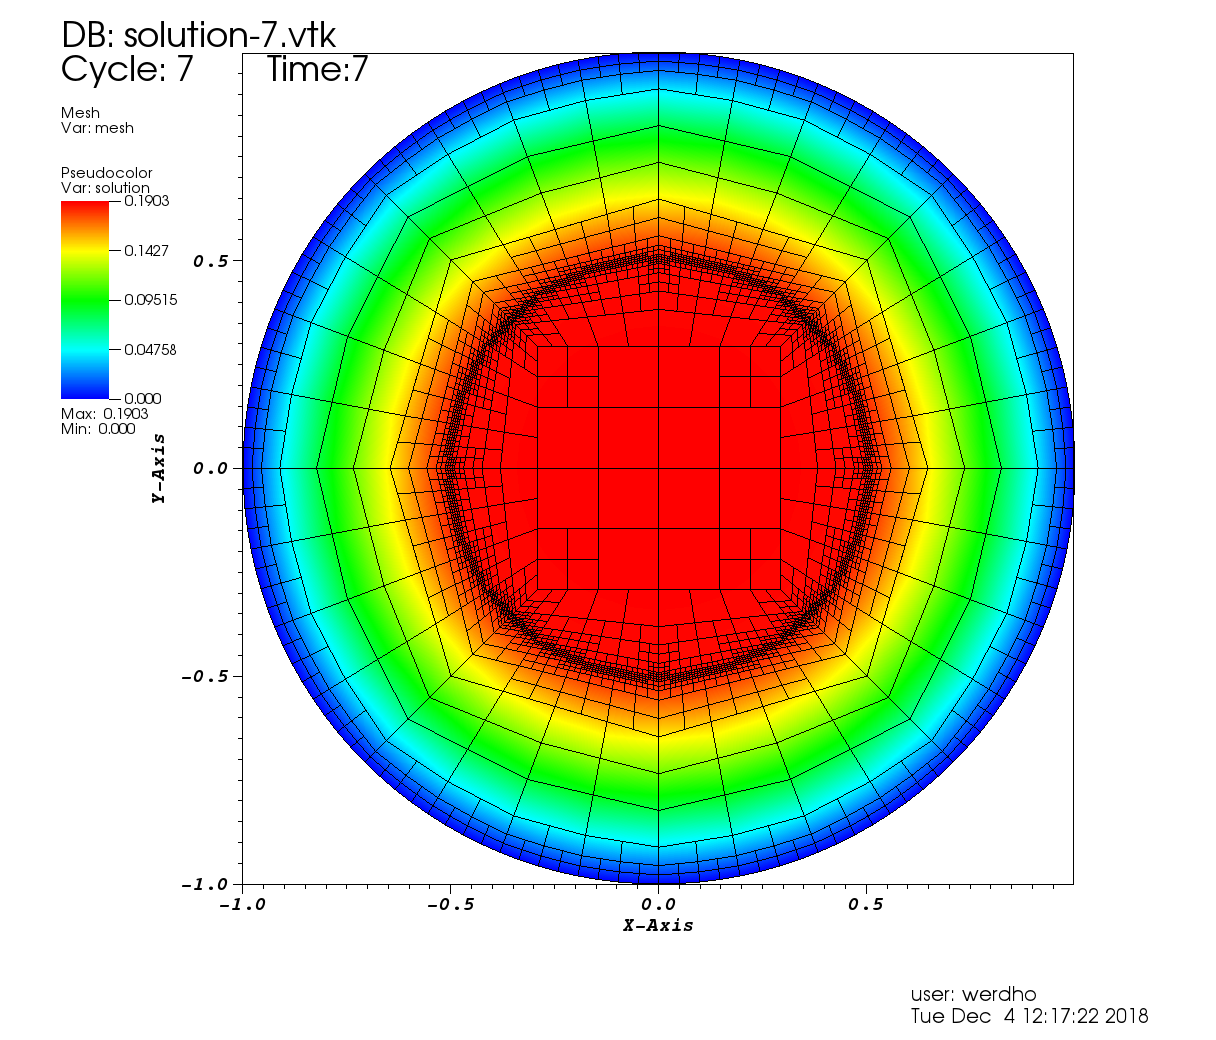
\includegraphics[scale=.12]{Step6-8.png}
	\end{minipage}
\end{figure}
\clearpage

\section*{Step-7}
In this tutorial we solved the Helmholtz equation:
$$
\begin{cases}
\Delta u + u = f &\text{in }\Omega\\
u = g_1 & \text{on }\Gamma_1 = \Gamma \cap \set{\set{x=1}\cup\set{y=1}},\\
\mathbf{n}\cdot \grad u = g_2 & \text{on }\Gamma_2 = \Gamma\setminus \Gamma_1
\end{cases}
$$
where $\Omega = [-1,1]^2$. The solution was chosen to be
$$
u(x) = \sum_{i=1}^3 \text{exp}\bigg(-\frac{\abs{x-x_i}^2}{\sigma^2}\bigg),
$$
with centers $x_1 = (-\frac{1}{2}, \frac{1}{2}), x_2=(-\frac{1}{2}, -\frac{1}{2}),(\frac{1}{2}, -\frac{1}{2})$ and $\sigma = \frac{1}{8}$. This choice of $u$ allowed us to compute the appropriate forcing function $f$ and BC $g_1, g_2$. Using this particular solution, we computed the $L^2$, $H^1$-semi, and $L^\infty$ error using global/adaptive refinement and $Q_1$ elements. Being able to compute the error and convergence rate will be useful in verifying our code for each of the three solvers individually before we try to incorporate them using the Picard iteration. Below are the error and convergence tables, and we note that the convergence rate matches what FEM theory tells us.

\begin{figure}[!ht]
	\centering
	\begin{tabular}{|c|r|r|c|c|c|} \hline
		cycle & \# cells & \# dofs & $L^2$-error & $H^1$-error &$L^\infty$-error\\ \hline
		0 & 64 & 81 & 1.629e+00 & 2.858e+00 & 1.683e+00\\ \hline
		1 & 256 & 289 & 3.563e-02 & 1.200e+00 & 1.324e-01\\ \hline
		2 & 1024 & 1089 & 1.196e-02 & 7.568e-01 & 7.901e-02\\ \hline
		3 & 4096 & 4225 & 3.049e-03 & 3.824e-01 & 2.343e-02\\ \hline
		4 & 16384 & 16641 & 7.661e-04 & 1.917e-01 & 6.109e-03\\ \hline
	\end{tabular}
	\caption{Error using global refinement and $Q_1$ elements.}
\end{figure}

\begin{figure}[!ht]
	\centering
	\begin{tabular}{|c|r|r|c|c|c|} \hline
		cycle & \# cells & \# dofs &$L^2$-error & $H^1$-error & $L^\infty$-error\\ \hline
		0 & 64 & 81 & 1.629e+00 & 2.858e+00 & 1.683e+00\\ \hline
		1 & 124 & 158 & 5.585e-02 & 1.201e+00 & 1.402e-01\\ \hline
		2 & 280 & 341 & 2.244e-02 & 7.925e-01 & 8.135e-02\\ \hline
		3 & 571 & 682 & 1.904e-02 & 5.185e-01 & 4.862e-02\\ \hline
		4 & 1087 & 1250 & 7.113e-03 & 3.097e-01 & 1.985e-02\\ \hline
		5 & 2122 & 2383 & 7.559e-03 & 2.191e-01 & 1.411e-02\\ \hline
		6 & 4051 & 4374 & 7.647e-03 & 1.543e-01 & 1.201e-02\\ \hline
		7 & 7699 & 8215 & 8.954e-03 & 1.134e-01 & 1.321e-02\\ \hline
		8 & 14749 & 15464 & 4.107e-03 & 8.716e-02 & 6.992e-03\\ \hline
	\end{tabular}
	\caption{Error using adaptive refinement and $Q_1$ elements.}
\end{figure}
\clearpage
\begin{figure}[!ht]
	\centering
	\begin{tabular}{|c|r|c|c|c|c|c|c|} \hline
		\multicolumn{2}{|c|}{n cells} & 
		\multicolumn{2}{|c|}{$H^1$-error} & 
		\multicolumn{2}{|c|}{$L^2$-error}\\ \hline
		0 & 64 & 2.858e+00 &  - & 1.629e+00 & -\\ \hline
		1 & 256 & 1.200e+00 &  1.25 & 3.563e-02 &  5.52\\ \hline
		2 & 1024 & 7.568e-01 &  0.66 & 1.196e-02 &  1.58\\ \hline
		3 & 4096 & 3.824e-01 &  0.99 & 3.049e-03 &  1.97\\ \hline
		4 & 16384 & 1.917e-01 &  1.00 & 7.661e-04 &  1.99\\ \hline
	\end{tabular}
	\caption{Estimated convergence using global refinement and $Q_1$ elements.}
\end{figure}


\section*{Step-8}
In this tutorial we solved the elastic equations:
$$
	\begin{cases}
	\partial_j(c_{ijkl}\partial_k u_l) = f_i, \quad i=1,...,d & \text{in }\Omega,\\
	u = 0 & \text{on } \partial \Omega,
	\end{cases}
$$
where $\Omega$ is the unit square or cube and
$$
	f_x(x) = \begin{cases}
	1 & x\in B((0,5,0), .2)\cup B((-0,5),.2),\\
	0 & \text{otherwise},
	\end{cases}\quad\quad
	f_y(x) = \begin{cases}
	1 & x\in B((0,0), .2),\\
	0 & \text{otherwise}.
	\end{cases}
$$
The new technique introduced was how to handle vector valued solutions. This will be useful as both the magnetization and the velocity of the fluid are vector valued.

\section*{Step-12}
In this tutorial we solved the linear advection equation:
$$
	\begin{cases}
	\grad\cdot(\beta u) = 0 \quad \text{on }\Omega,\\
	u = g & \text{on } \Gamma_1-,
	\end{cases}
$$
where $\Omega = [0,1]^2$, $\beta = \frac{1}{\abs{x}}(-x_2,x_1)$, $\Gamma_- = \set{x\in\partial\Omega | \beta(x)\cdot \eta(x) < 0}$, and $g=1$. This problem was solved using discontinuous elements, in order to use an upwinding technique for the advection equation. This tutorial demonstrated how to handle integrals over faces of edges, which will be useful when solving the magnetization equation (even though the bilinear form will be different than the one presented in this tutorial).

\section*{Step-20}
In this tutorial we solved Stokes equation:
$$
\begin{cases}
K^{-1}\mathbf{u} + \grad p = 0 &\text{in }\Omega\\
-\text{div}\mathbf{u} = -f & \text{in }\Omega\\
p = g & \text{on }\partial \Omega,
\end{cases}
$$
where $K$ was chosen to be the identity. We chose the exact solution to be
$$
p = -\bigg(\frac{\alpha}{2}xy^2 + \beta x - \frac{\alpha}{6}x^3\bigg), \quad \mathbf{u} = \begin{pmatrix}
\frac{\alpha}{2}y^2 + \beta - \frac{\alpha}{6}x^2\\
\alpha xy
\end{pmatrix}.
$$
The above system is a saddle point system and was solved using a Schur complement technique. The interesting technique shown was that we don't actually need to compute the Schur complement, but instead just need to know its action on a vector. Additionally, a method for preconditioning the Schur complement was discussed. This technique will be used to solve the Navier--Stokes system, albeit with a more advanced preconditioner. Below is a plot of the magnitude of the solution.

\begin{figure}
	\centering
	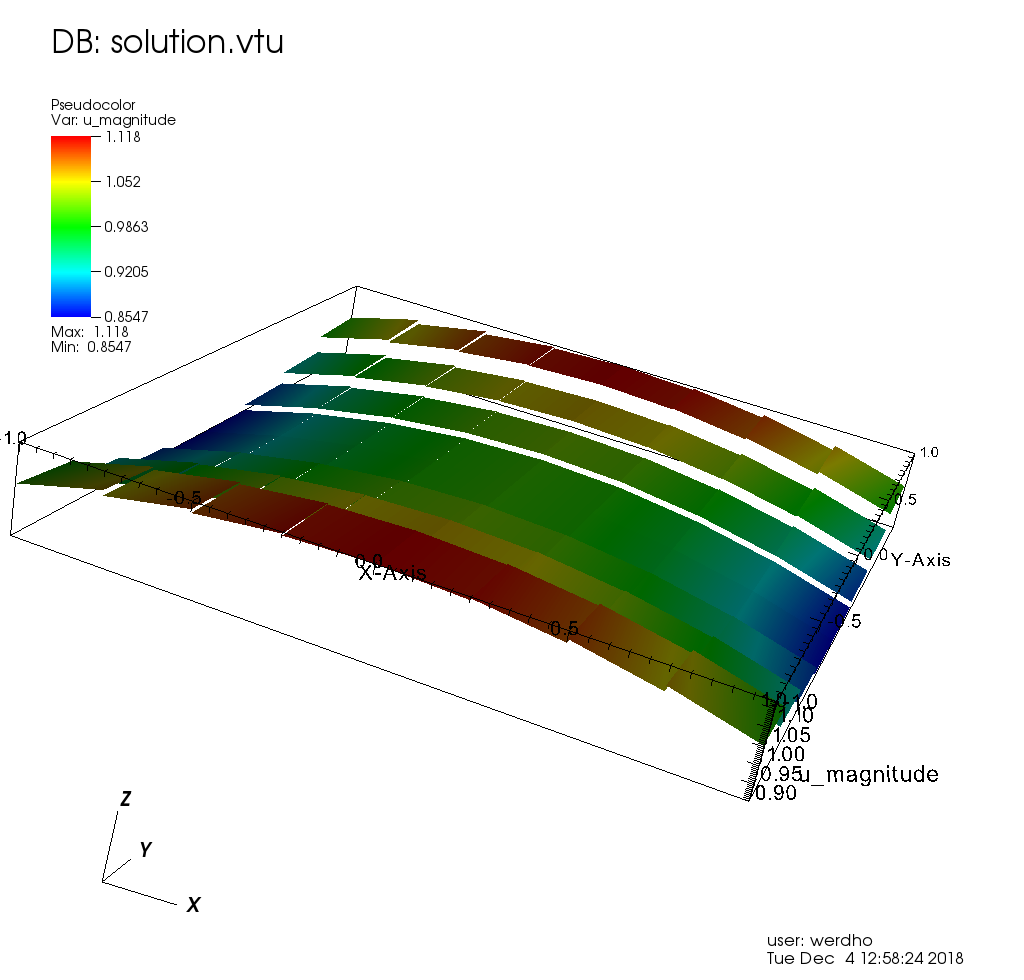
\includegraphics[scale=.25]{Step20.png}
\end{figure}

\section*{Step-26}
In this tutorial we solved the heat equation:
$$
\begin{cases}
\partial_t u(x,t) -\Delta u(x,t) = f(x,t) &\text{in }\Omega\times (0,1]\\
u(x,0) = u_0(x) & \text{on } \Omega \times \set{0}\\
u(x,t) = g(x,t) & \text{on }\text{on }\partial\Omega\times (0,1].
\end{cases}
$$
The solution was chosen to be
$$
u(x,y,t) = \sin(3\pi x)e^{-y-2t}.
$$
Two main techniques were introduced. The first was how to handle time dependent problems. By using a theta-scheme, we were able to discretize the PDE in time with $\theta=1$ corresponding to Backward Euler, $\theta = 0$ corresponding to Forward Euler, and $\theta = .5$ corresponding to Crank-Nicholson. Second, a method for adaptive refinement/coarsening for time dependent problems was discussed. The mesh is refined/coarsened at a fixed interval of time steps, using the same refinement technique shown in previous examples. The main issue with this is that the DoFs on the two meshes will be different and thus you will need to interpolate the solution from one mesh to the other. Both of the techniques presented in this tutorial will be used almost exactly in our implementation for each of the three solvers. Movies of both the mesh and solution for the PDE are given in the folder Examples/step-26.

\bibliographystyle{siam}
\bibliography{ExampleCodeDocumentation}

\end{document}
